\documentclass[tikz,border=5]{standalone}

\usepackage{tikz}
\usetikzlibrary{positioning}
\usetikzlibrary{calc}

\makeatletter 

\tikzset{curlybrace/.style={rounded corners=2pt,line cap=round}}%  
\pgfkeys{% https://tex.stackexchange.com/a/45129/121799
/curlybrace/.cd,%
tip angle/.code     =  \def\cb@angle{#1},
/curlybrace/.unknown/.code ={\let\searchname=\pgfkeyscurrentname
                              \pgfkeysalso{\searchname/.try=#1,
                              /tikz/\searchname/.retry=#1}}}  
\def\curlybrace{\pgfutil@ifnextchar[{\curly@brace}{\curly@brace[]}}%

\def\curly@brace[#1]#2#3#4{% 
\pgfkeys{/curlybrace/.cd,
tip angle = 0.75}% 
\pgfqkeys{/curlybrace}{#1}% 
\ifnum 1>#4 \def\cbrd{0.05} \else \def\cbrd{0.075} \fi
\draw[/curlybrace/.cd,curlybrace,#1]  (#2:#4-\cbrd) -- (#2:#4) arc (#2:{(#2+#3)/2-\cb@angle}:#4) --({(#2+#3)/2}:#4+\cbrd) coordinate (curlybracetipn);
\draw[/curlybrace/.cd,curlybrace,#1] ({(#2+#3)/2}:#4+\cbrd) -- ({(#2+#3)/2+\cb@angle}:#4) arc ({(#2+#3)/2+\cb@angle} :#3:#4) --(#3:#4-\cbrd);
}
\makeatother

\begin{document}

    \centering      
    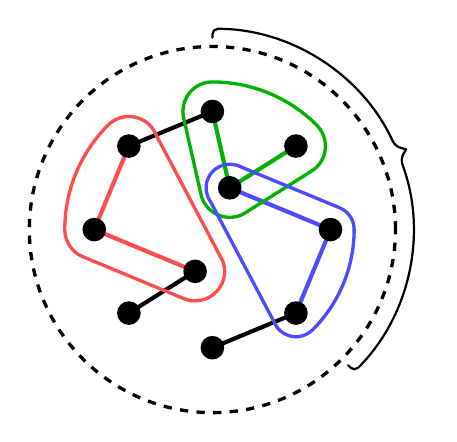
\begin{tikzpicture}[scale=1.5,
    myline/.style={line width=1.5}
    ]

    %% Setting coordinates
    \foreach \n in {1,...,8}{
        \coordinate (P\n) at (\n*45:1);
    }
    \coordinate (P9) at ($.5*(P3)+.5*(P8)$);
    \coordinate (P10) at ($.5*(P4)+.5*(P7)$);

    %% Drawing the graph
    \draw[myline,blue!70] (P7) -- (P8) -- (P9);
    \draw[myline,red!70] (P3) -- (P4) -- (P10);
    \draw[myline,green!70!black] (P1) -- (P9) -- (P2);
    \draw[myline] (P5) -- (P10);
    \draw[myline] (P6) -- (P7);
    \draw[myline] (P2) -- (P3);

    %% Drawing the shapes
    \draw[dashed, very thick] (0,0) circle (1.55);
    \curlybrace[tip angle=-2,thick]{90}{-45}{1.7}
    \draw[green!70!black, very thick] (45:1.25) arc (45:90:1.25) arc (90:190:.25)
    -- ($(P9)+(-170:.25)$) arc (-170:-55:.25)
    -- ($(P1)+(-55:.25)$) arc (-55:45:.25);

    \draw[red!70, very thick] (135:1.25) arc (135:180:1.25) arc (180:250:.25)
    -- ($(P10)+(250:.25)$) arc (250:380:.25)
    -- ($(P3)+(20:.25)$) arc (20:135:.25);

    \draw[blue!70, very thick] (-45:1.2) arc (-45:0:1.2) arc (0:70:.2)
    -- ($(P9)+(70:.2)$) arc (70:215:.2)
    -- ($(P7)+(215:.2)$) arc (215:315:.2);

    %% Drawing the node
    \foreach \n in {1,...,10}{
        \fill (P\n) circle (.1);
    }
    
    \end{tikzpicture}       
\end{document}